%!TEX root = ../report.tex
\documentclass[../report.tex]{subfiles}

\begin{document}
    \section{Experimental Approach}
    This section describes the experimental approach to developing and modeling a training pipeline for terrain segmentation from the 3-D point cloud LiDAR dataset. This approach consists of several steps, including data collection, pre-processing, evaluation, validation, and finally, the conclusion based on the experiments.
    
    \subsection{Tools and Environment Setup}
    The project environment was established using Anaconda to ensure reproducibility and consistency. A dedicated environment with all dependencies was maintained and shared via GitHub\cite{github}. Core tools included CloudCompare\cite{CloudCompare} for 3D point cloud visualization and preprocessing, Open3D for Python-based processing, and MATLAB\cite{matlab} for supplementary analysis. SciKit-learn supported clustering and data preprocessing, while the PCL (Point Cloud Library)\cite{PCL} was employed for specialized point cloud operations during experimentation.

    \subsection{Data Pre-Processing}
    The initial dataset comprised 3D LiDAR point clouds of Field-D, captured by the Garrulus team’s UAV in a local coordinate system, without georeferencing or RGB data. It included point clouds, polygon meshes, and VTK files. A 100×100×100 m Region of Interest (ROI) was selected using CloudCompare for focused analysis, and exported as a polygon mesh for better cross-platform compatibility.

    The dataset contained several invalid points (NaN and infinite), which were retained but ignored during processing in Open3D to avoid loss of potentially useful information. Further cropping was done based on visible fencing boundaries, and the cleaned polygon mesh was finalized as a benchmark for subsequent processing and experiments.
    
    \subsection{Segmentation & Clustering Techniques}

    To segment meaningful structures from the filtered point cloud data, the Density-Based Spatial Clustering of Applications with Noise (DBSCAN)\cite{DBSCan_Grammarly} algorithm was employed. DBSCAN is particularly well-suited for 3D point cloud segmentation due to its ability to identify arbitrarily shaped clusters and its robustness to noise. The input point cloud, stored in .ply format, was loaded using the Open3D library and converted into a NumPy array to facilitate clustering using the scikit-learn implementation of DBSCAN.
    
    Clustering was performed using a rich set of features: in addition to the basic spatial coordinates (x, y, z), geometric descriptors such as surface normals (nx, ny, nz), curvature, and local point density were included. These additional features, which are critical for distinguishing between different natural elements like tree stumps, terrain, and undergrowth, added contextual information beyond mere location. This multi-dimensional feature space allowed DBSCAN to more accurately group points with similar geometric and structural characteristics.
    
    The DBSCAN parameters were tuned to the nature of the dataset, with an epsilon\cite{dbscan_eps} (EPS) value of 0.05 and a minimum samples threshold of 800, balancing sensitivity to dense clusters and resistance to outliers. Points were assigned cluster labels, with label -1\cite{dbscan_eps2} indicating noise. Clusters were visualized using the jet colormap from Matplotlib, with each cluster assigned a unique color and noise points shown in black, providing an intuitive and informative 3D visualization using Open3D’s interactive viewer.
    
    This technique is especially beneficial in natural, unstructured environments—such as the forests familiar from UAV scans—where distinguishing fine features like tree stumps or ground depressions can be vital. Individual clusters, such as the largest one (often corresponding to terrain), could be isolated for deeper analysis, enabling a targeted examination of ecological or structural elements within the scene.
        
	\subsection{Challenges Faced}
    One of the significant challenges faced during this project was the absence of labeled data in the LiDAR point cloud. Manual annotation of the point cloud data became a significantly time-consuming task without prior labeling and no direct reference to photogrammetry or RGB values. Additionally, directly labeling the point cloud would have resulted in a compromise of precision and accuracy due to the complicatedness in visually distinguishing between objects using only geometric features.

    Two auxiliary methods were introduced to address this issue. During data acquisition, the UAV system simultaneously captured both LiDAR and RGB photogrammetry data. The RGB data, being more intuitive for human interpretation, was manually annotated using QGIS. These annotations were then exported in the GeoPackage\cite{gdal2025gpkg} (.gpkg) format, which allowed for high-resolution spatial referencing and integration with other datasets.
    
    A secondary challenge involved the disparity in coordinate systems. The RGB photogrammetry data was geo-referenced, aligning with a global spatial reference system, whereas the LiDAR data was captured using a local coordinate system. However, due to the availability of metadata and known reference points, it was feasible to transform both datasets into a unified, standardized coordinate system. This enabled accurate overlay and cross-referencing between the manually labeled photogrammetry data and the LiDAR point cloud, ultimately improving the efficiency and reliability of the labeling process.
    \begin{figure}[H]
        \centering
        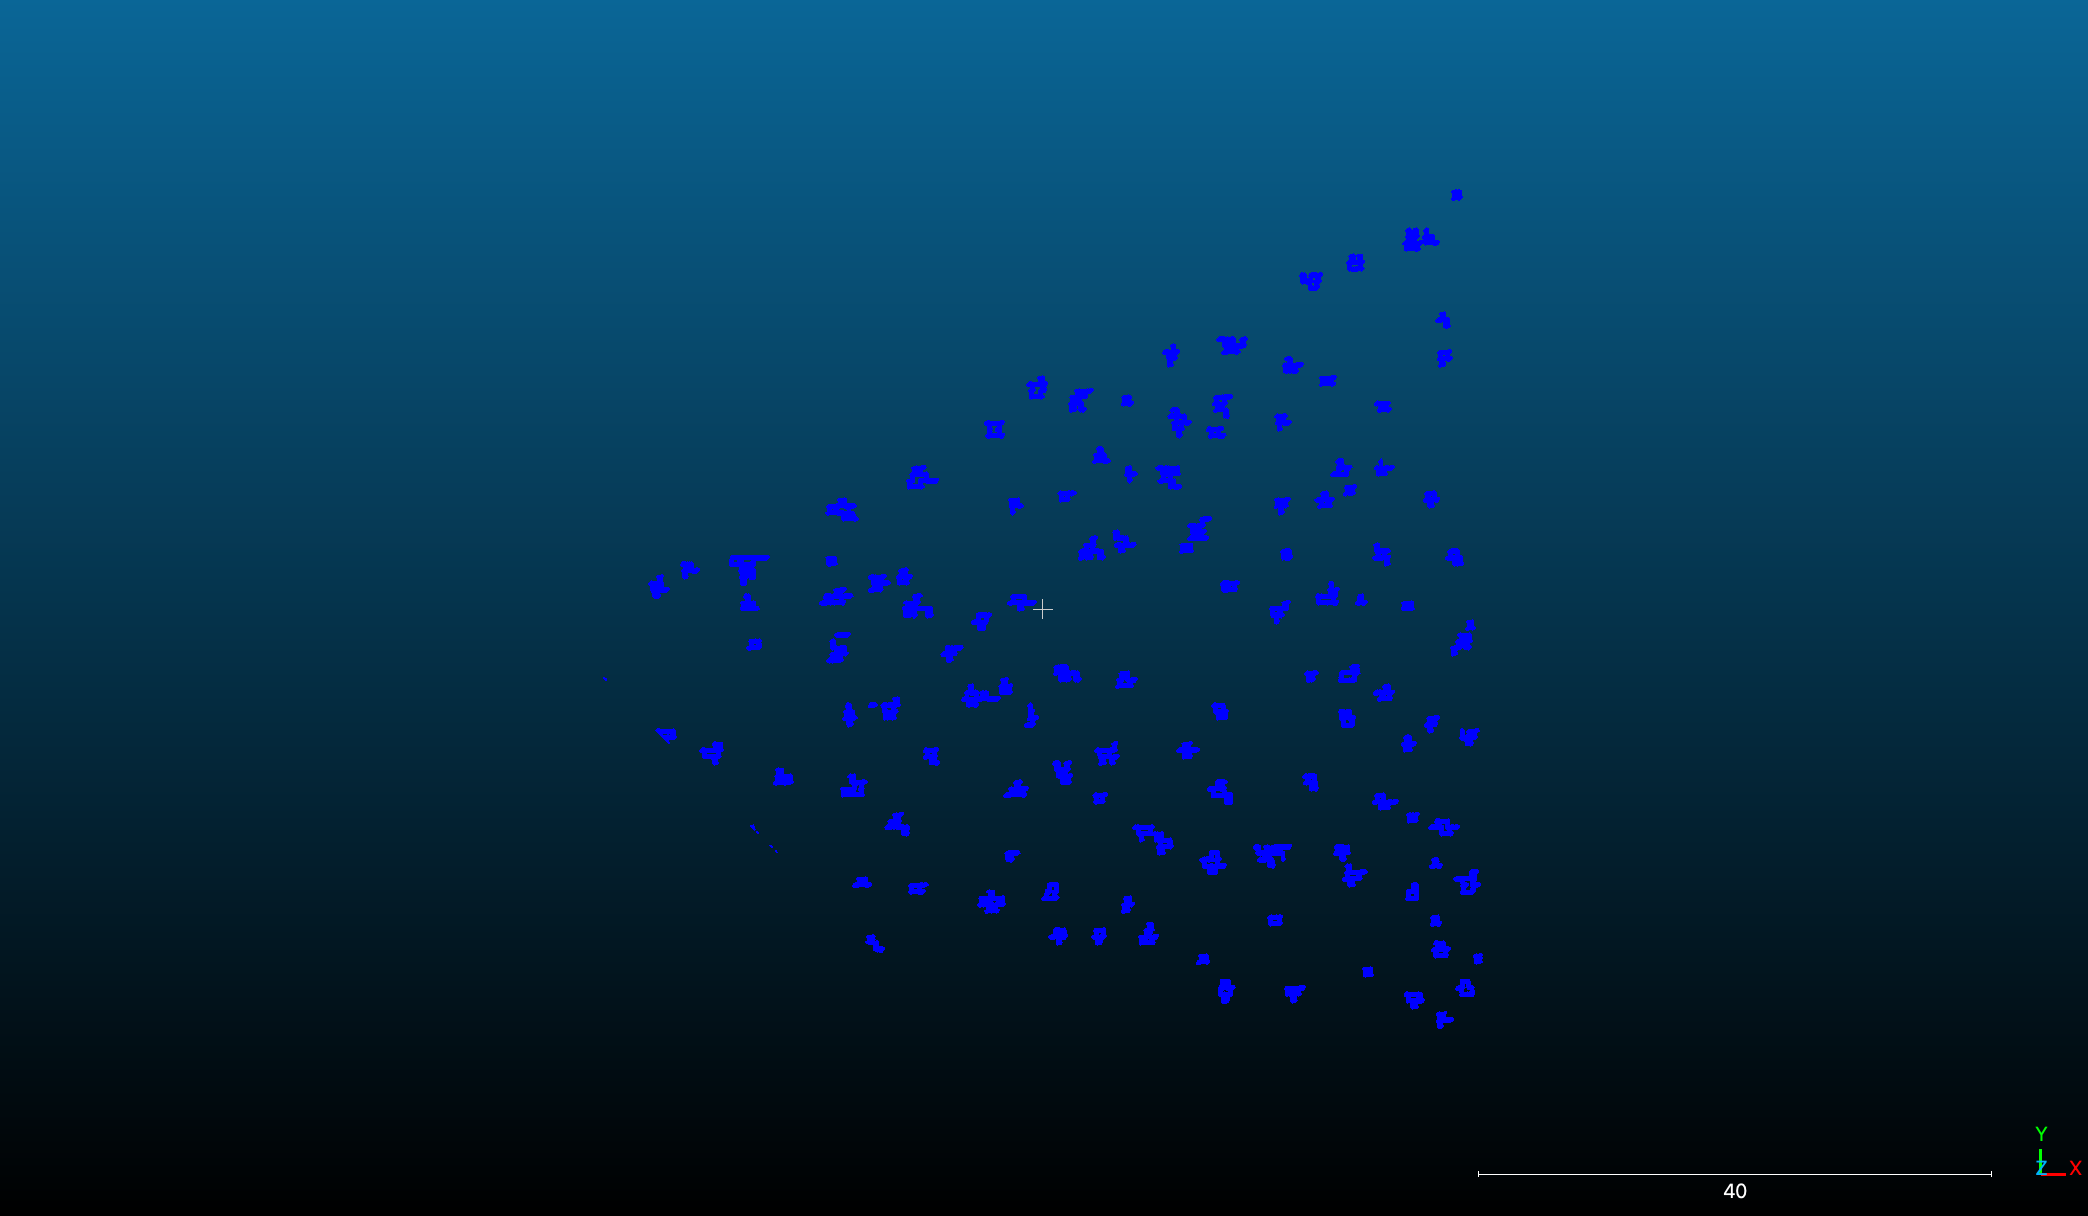
\includegraphics[width=0.4\textwidth]{rnd-project-report-main/figures/Stumps_matched.png}
        \caption{Stumps}
        \label{fig:stumps}
    \end{figure}
    
    
	\subsection{Data Preparation}
    Following the collection of the LiDAR datasets and their corresponding RGB photogrammetry data, along with the associated GeoPackage (.gpkg) annotations, the next critical step was extracting and aligning semantic labels. Although the GeoPackage format provided precise 2D polygonal annotations—particularly for features like tree stumps—aligning these 2D labels\ref{fig:stumps} with the 3D LiDAR data posed a significant challenge. The process required accurately mapping flat polygonal data to volumetric point clouds, a task complicated by the lack of direct height information.

    To bridge this dimensional gap, an approximate height of 0.3 meters was assumed for stump structures based on field observations and average stump dimensions. This approximation enabled the transformation of 2D annotations into 3D labeled regions, which were then converted into .ply format to ensure compatibility with LiDAR processing tools. Subsequent alignment of the converted 3D labels with the point cloud was performed using reference-based registration and Iterative Closest Point (ICP) algorithms available in CloudCompare. This step ensured spatial accuracy between labeled regions and the actual 3D geometry of the environment.
    
    The labeled dataset was segmented into square grid tiles upon successful alignment to facilitate model training and evaluation. Each grid was assigned one of three class labels based on the contents of the points within it: 0 for terrain, 1 for stumps, and 2 for all other elements. Several permutations were tested to determine the optimal grid size. After extensive trials, a 7×7 meter grid size was selected as it provided a balanced distribution of points across categories while maintaining spatial resolution sufficient for effective classification and segmentation tasks.\ref{tab:datasample}
    
	\subsection{Model Experiments}
    The prepared dataset, originally in CSV format, contained key geometric and structural attributes, including the x, y, and z coordinates, surface normals, curvature values, and class labels. To facilitate deep learning experiments using PointNet and PointNet++ architectures, the dataset was converted into formats compatible with each model’s input requirements.

    For the classification task using PointNet, the dataset was transformed into NumPy (.npy) arrays. The data was then organized into labeled directories corresponding to each class. A stratified split was performed to divide the dataset into training and testing subsets, allocating 70\% of the samples for training and the remaining 30\% for testing. These structured inputs were then fed into the PointNet classification model to evaluate its ability to distinguish between terrain, stumps, and other features based on point cloud geometry.
    
    In the case of PointNet++ for segmentation tasks, the dataset was formatted as 6×N matrices, where each column represented a single point consisting of x, y, and z coordinates referring to labels, curvature, and density. These were also stored in .npy format for compatibility with the model architecture. This configuration enabled the network to perform point-wise classification across the entire spatial domain, allowing fine-grained segmentation of the forest environment.
	%8.	Conclusion & Future Work
    

\end{document}
%     Describe all conceptual details about your approach in this section.
%     Add any necessary subsections to improve the presentation.

%     Feel free to rename this section to better reflect the concrete topic you are discussing.
% \end{document}
